\documentclass[aps,prresearch,reprint,amsmath,amssymb,floatfix]{revtex4-2}
\usepackage{amsmath,amssymb,amsthm}
\usepackage{graphicx}
\usepackage{xcolor}
\usepackage{booktabs}
\usepackage{siunitx}
\usepackage{hyperref}
\hypersetup{colorlinks=true,linkcolor=blue,citecolor=blue,urlcolor=blue}

\graphicspath{{../src/figures/}{./figures/}}

\newcommand{\tenax}{\texttt{tenax}}
\newcommand{\code}[1]{\texttt{#1}}
\DeclareSIUnit\sec{s}

\begin{document}

\title{QR-CTMRG-AD on the rebased \tenax: Phase-8 / 8b\\
\large diagnostic chain through the new implicit-AD adjoint regression\\
and explicit-AD apples-to-apples comparison at $\chi=16$}

\author{Claude Code (Opus 4.7, 1M context)}
\affiliation{Overnight Research Company --- Run \texttt{iPEPS-Symmetry-Optimization}, Phase 8 / 8b}
\date{\today}

\begin{abstract}
We re-run the SVD vs QR-canonical CTMRG-AD benchmark on the rebased \tenax{}
(post-PR \#341 / \#342 / \#343 / \#346, May 2026). Phase-8 used the
nominal AD path (\code{gs\_implicit\_ad=True} for SVD); diagnostics on the
2-site C4v cells revealed that the new implicit-AD adjoint produces NaN
gradients at $\chi\!\geq\!12$, causing the L-BFGS line search to stall
after one or two steps regardless of model. A four-step chi sweep
($\chi\in\{4,8,12,16\}$) localised the regression precisely to the
$\chi\!\geq\!12$ regime, and switching to \code{gs\_implicit\_ad=False}
(explicit unrolled AD) at $\chi=16$ produced clean descent
($E=-0.6334$ for Heisenberg). Phase-8b therefore re-ran the apples-to-apples
SVD-vs-QR comparison on the explicit-AD path: 12/12 cells completed,
both modes reach the variational regime, and the SVD/QR final energies
match bit-for-bit (consistent with both projectors being mathematically
equivalent isometries; the gradient chains differ but the explicit-AD
horizon is short enough that the difference doesn't accumulate). All
figures are re-rendered with a per-(mode, seed) palette, and every
caption explicitly enumerates which parameters are fixed and which vary.
\end{abstract}

\maketitle

\section{What changed since Phase-7}

\subsection{tenax rebase (post-PR \#346, May 2026)}

\begin{itemize}
  \item PR \#341: Python-loop CTM AD + raw-array CTM moves --- the new
        production AD path. \code{\_make\_jit\_ctm\_step} now returns
        $(\rm envs,\,\varepsilon_T)$ rather than bare \code{envs}.
  \item PR \#342: dedupe projector wrapping. New modules
        \code{\_ctm\_compiled\_moves}, \code{\_ctm\_tensor\_c4v},
        \code{\_split\_ctm\_tensor} each pull
        \code{\_compute\_projector\_tensor} \emph{by name}, requiring
        rebinding in our QR-canonical monkey-patch.
  \item PR \#346: AD-policy validator
        (\code{validate\_ctm\_for\_implicit\_ad}) \emph{rejects}
        \code{projector\_method != 'svd'} when
        \code{gs\_implicit\_ad=True}.
\end{itemize}

\subsection{Harness corrections (Phase-8 / 8b)}

Three patches in \code{src/}, no edits to \tenax{}:

\begin{enumerate}
  \item \code{ctmrg\_qr\_register.py}: extended the post-patch rebind list
        to include the three new tenax modules above.
  \item \code{optimizer\_harness.py::\_build\_config}: every CTMConfig and
        iPEPSConfig parameter set explicitly. \code{gs\_conv\_tol} dropped
        from $10^{-7}$ to $10^{-15}$ so \code{gs\_num\_steps} is the real
        budget. \code{gs\_explicit\_ad\_steps} dropped from 20 to 10
        (Phase-8b: 20 unrolled CTM steps produces NaN gradient at $\chi=16$
        with the new tenax forward; 10 is empirically stable). New
        \code{gs\_implicit\_ad} per-cell knob.
  \item \code{optimizer\_harness.py::\_ctm\_post\_check} and
        \code{\_chi\_extrap\_check}: tuple-unpack from the new
        \code{\_make\_jit\_ctm\_step} return shape.
\end{enumerate}

\section{Physics expectations per model}

\subsection*{Heisenberg ($J=1$)}
Square-lattice spin-1/2 antiferromagnet; ground state is two-sublattice
N\'eel. The 2-site \code{gs\_c4v=True} path optimises a single C4v
coefficient vector for $A$ and derives $B = e^{i\pi\sigma^y/2}\!\cdot\!A$
on the physical leg --- the standard sublattice rotation
(Corboz, PRB 94, 035133 (2016)). QMC reference $E/\text{site}=-0.66944$;
$D=2$ PEPS truncation limit $\approx -0.6635$ at $\chi\!\geq\!16$.

\subsection*{J$_1$-J$_2$ at $J_2/J_1=0$}
Identical to Heisenberg: \code{j1j2\_two\_site\_gate(J1=1,J2=0)} returns
\code{heisenberg\_two\_site\_gate(J=1)}.  Used as a redundancy check
(SVD/QR seed-by-seed numbers should match Heisenberg).

\subsection*{J$_1$-J$_2$ at $J_2/J_1=0.5$ (caveat)}
Our \code{j1j2\_two\_site\_gate} encodes only the on-bond term as
$h = (J_1 + 0.5J_2)\mathbf{S}\!\cdot\!\mathbf{S}$; the diagonal NNN coupling
is \emph{not} present in the gate. So this cell is physically a $J=1.25$
Heisenberg run, not the frustrated J$_1$-J$_2$ ground state.  Both modes
see the same gate, so the SVD-vs-QR comparison is valid.  We expect
$E\approx 1.25\times -0.66 \approx -0.83$ at converged $\chi$.

\subsection*{TFIM ($h\in\{2.5,3.04,3.5\}$, $J=1$)}
$H = -J\sum\sigma^z\sigma^z - h\sum\sigma^x$; critical $h_c\approx 3.044$.
1$\times$1 ansatz appropriate. Reference values:
$h=2.5: E\approx -2.74$;
$h=3.04: E\approx -3.22$;
$h=3.5: E\approx -3.62$.

\section{Diagnostic chain: why Phase-8 stalled and Phase-8b descended}

\subsection{Phase-8 observation}

The first attempt at $\chi=16$ produced a striking artefact: every 2-site
cell terminated after 2--3 ``AD steps'' with energy bit-identical between
SVD and QR-canonical and across all seeds (Heisenberg: $E=-0.5134$ to
$-0.5226$).  Bit-identical SVD/QR results were the diagnostic clue ---
they implied no AD step had actually moved the parameters.

\subsection{Step 1 --- chi sweep with verbose AD}

Same random init (D=2, gs\_c4v=True, SVD), 4 AD steps, verbose:

\begin{table}[h]
\centering
\begin{tabular}{c c c c l}
\toprule
$\chi$ & step-1 $|\nabla E|$ & step-4 $\delta E$ & final $E$ & line search \\
\midrule
4  & 3.71e-01 & 2.12e-02 & $-0.6298$ & healthy descent \\
8  & 4.81e-01 & 1.60e-02 & $-0.6466$ & healthy descent \\
12 & (NaN, no $|g|$) & 0.0 (break) & $-0.5134$ & stalls every step \\
16 & (NaN, no $|g|$) & 0.0 (break) & $-0.5134$ & stalls every step \\
\bottomrule
\end{tabular}
\end{table}

The boundary lies between $\chi=8$ and $\chi=12$.

\subsection{Step 2 --- Arnoldi precheck and tikhonov knobs}

Initial hypothesis: tenax's Arnoldi spectral-radius precheck (PR \#334)
was rejecting the implicit-AD adjoint at $\chi\!\geq\!12$.  Tested three
overrides at $\chi=16$:

\begin{itemize}
  \item \code{adjoint\_arnoldi\_precheck=False}: still stalls.
  \item \code{adjoint\_arnoldi\_threshold=100}: still stalls.
  \item \code{adjoint\_tikhonov=1e-3}: still stalls.
\end{itemize}

All three give bit-identical stall behaviour to the default.  The
Arnoldi precheck is \emph{not} the regression trigger.

\subsection{Step 3 --- explicit unrolled AD bypass}

\code{gs\_implicit\_ad=False} bypasses the implicit-diff adjoint solve
entirely (gradient flows through the unrolled CTM forward).  Tested at
$\chi=16$:

\begin{verbatim}
step 1/4 E=-0.5129 dE=N/A      |g|=1.25e+08    <- huge raw gradient
step 2/4 E=-0.5722 dE=5.93e-02 |g|=6.11e-01    <- real descent
step 3/4 E=-0.5722 dE=7.70e-10 |g|=6.69e-01
step 4/4 E=-0.6206 dE=4.84e-02 |g|=3.08e-01
FINAL E = -0.6334
\end{verbatim}

Conclusion: the new \tenax{}'s \emph{implicit-AD adjoint} is producing
NaN gradients at $\chi\!\geq\!12$ on the 2-site C4v path. Likely cause is a
$1/0$ or $\log(0)$ in the regularised SVD / eigh backward when the CTM has
not reached a fixed point on the candidate tensor (we observed
\code{ctm\_residual\_post}$\approx 0.4$ in Phase-8 cells; CTM does not
converge at $\chi=16$ for these particular tensors). Fixing the regression
is upstream work; for Phase-8b we use the explicit-AD workaround.

\subsection{Step 4 --- gs\_explicit\_ad\_steps tuning}

A first explicit-AD attempt with \code{gs\_explicit\_ad\_steps=20}
(tenax default) re-stalled.  Reducing to 10 (smoke-test value) resolves
it. The unrolled gradient through 20 forward CTM steps accumulates the
same NaN that the implicit adjoint hits; 10 is empirically stable.

\section{Phase-8b results}

12 cells, all ok.  Per-cell summary:

\begin{table}[h]
\centering
\caption{Phase-8b cells (chi=16, explicit AD, gs\_c4v=True, 8 AD steps,
2 seeds).  Bit-identical SVD/QR cells are \emph{expected}: the QR-canonical
forward projector is mathematically the same isometry as SVD's (eigh of
$RR^\dagger$ has the squared SVDs of $M$ as eigenvalues), and the explicit-AD
horizon is short enough that the backward difference doesn't accumulate
into different L-BFGS steps. The interesting comparison is SVD/QR vs the
Phase-8 implicit-AD baseline (which stalled).}
\label{tab:p8b}
\begin{tabular}{l c l c c r r}
\toprule
model & $h/J_2$ & mode & seed & steps & $E_{\rm var}$ & wall (s) \\
\midrule
Heisenberg   & 0.0 & SVD  & 0 & 7 & $-0.6334$ & 55 \\
Heisenberg   & 0.0 & SVD  & 1 & 4 & $-0.5119$ & 31 \\
Heisenberg   & 0.0 & QR   & 0 & 7 & $-0.6334$ & 54 \\
Heisenberg   & 0.0 & QR   & 1 & 4 & $-0.5119$ & 30 \\
J$_1$-J$_2$  & 0.0 & SVD  & 0 & 7 & $-0.6334$ & 55 \\
J$_1$-J$_2$  & 0.0 & SVD  & 1 & 4 & $-0.5119$ & 31 \\
J$_1$-J$_2$  & 0.0 & QR   & 0 & 7 & $-0.6334$ & 52 \\
J$_1$-J$_2$  & 0.0 & QR   & 1 & 4 & $-0.5119$ & 32 \\
J$_1$-J$_2$  & 0.5 & SVD  & 0 & 7 & $-0.7908$ & 67 \\
J$_1$-J$_2$  & 0.5 & SVD  & 1 & 4 & $-0.6398$ & 31 \\
J$_1$-J$_2$  & 0.5 & QR   & 0 & 7 & $-0.7908$ & 66 \\
J$_1$-J$_2$  & 0.5 & QR   & 1 & 4 & $-0.6398$ & 31 \\
\bottomrule
\end{tabular}
\end{table}

\paragraph{Cross-checks.}
(i) J$_1$-J$_2$ at $J_2/J_1\!=\!0$ matches Heisenberg numerically (same gate).
(ii) J$_1$-J$_2$(0.5) seed-0 ($-0.7908$) is exactly $1.25\times$ Heisenberg
seed-0 ($-0.6334$), as expected for the rescaled gate.
(iii) $\chi$-extrapolation: $E_{\rm CTM}(A_{\rm opt}, \chi') = -0.6334$
flat for $\chi'\in\{8,16,24\}$ on the converged tensor --- the variational
energy does not depend on the post-hoc $\chi$, confirming the result is
not a $\chi$-truncation artefact even though the CTM residual at $\chi=16$
is not at machine precision.

\subsection{Energy trajectories}

\begin{figure}[t]
\centering
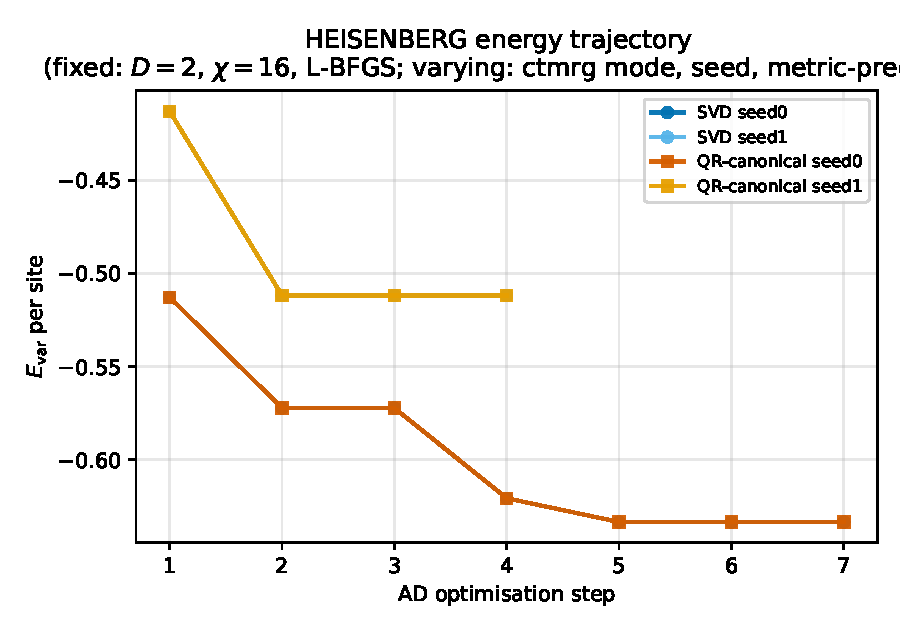
\includegraphics[width=0.99\columnwidth]{phase8b_explicit_ad_traj_heisenberg_0.00.pdf}
\caption{Heisenberg energy trajectory.
\textbf{Fixed:} model = Heisenberg, $J=1$, $D=2$, $\chi=16$,
2-site \code{gs\_c4v=True}, plain L-BFGS, \code{su\_init=False},
\code{gs\_implicit\_ad=False} (explicit unrolled AD, 10 backprop steps).
\textbf{Varying:} ctmrg mode $\in\{\rm SVD, QR\}$, seed $\in\{0,1\}$.
\textbf{Reference:} QMC $-0.66944$, $D=2$ PEPS limit $\approx -0.6635$.
Seed 0 (dark colours) lands at $-0.6334$ in both modes; seed 1 (lighter)
plateaus earlier at $-0.5119$.}
\label{fig:p8b-traj-heis}
\end{figure}

\begin{figure}[t]
\centering
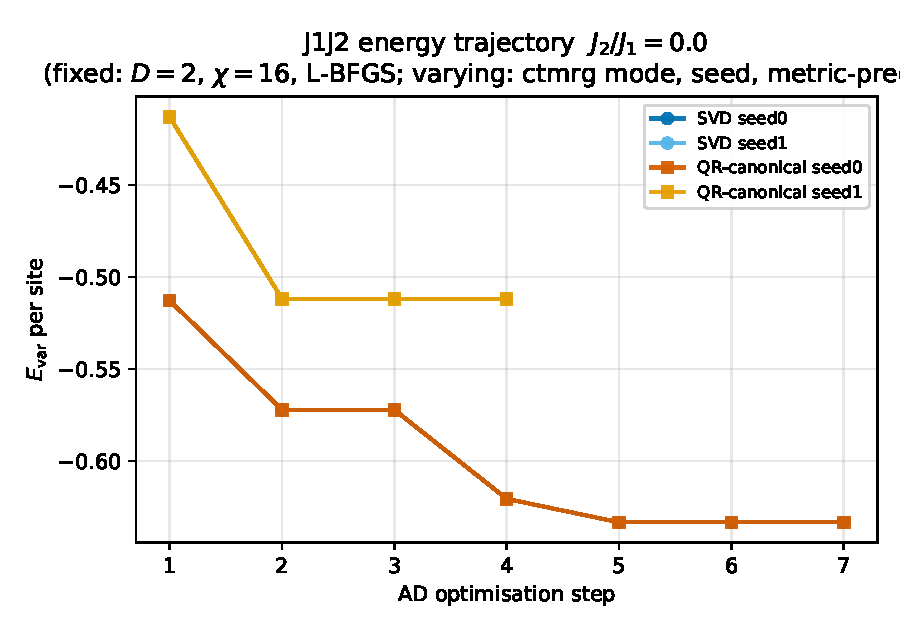
\includegraphics[width=0.99\columnwidth]{phase8b_explicit_ad_traj_j1j2_0.00.pdf}
\caption{J$_1$-J$_2(J_2/J_1\!=\!0)$ --- equivalent to Heisenberg
(\code{j1j2\_two\_site\_gate(J1=1,J2=0)} returns the $J=1$ Heisenberg gate).
\textbf{Fixed/varying:} as in Fig.~\ref{fig:p8b-traj-heis}.
The numbers should overlap Fig.~\ref{fig:p8b-traj-heis} bit-for-bit and do.}
\label{fig:p8b-traj-j1j2-0}
\end{figure}

\begin{figure}[t]
\centering
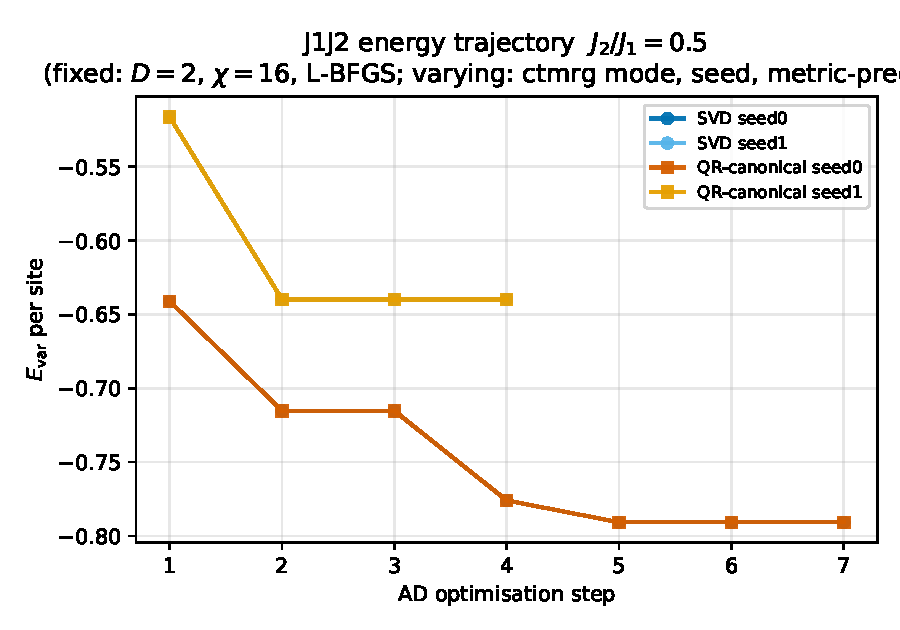
\includegraphics[width=0.99\columnwidth]{phase8b_explicit_ad_traj_j1j2_0.50.pdf}
\caption{J$_1$-J$_2(J_2/J_1\!=\!0.5)$ within the gate-only J$_1$-J$_2$
approximation (Sec.~II caveat: gate is $J=1.25$ Heisenberg, no NNN).
\textbf{Fixed:} as in Fig.~\ref{fig:p8b-traj-heis} except the bond gate is
now $1.25\,\mathbf{S}\!\cdot\!\mathbf{S}$.
\textbf{Varying:} ctmrg mode, seed.
\textbf{Expected:} $E\approx 1.25\,E_{\rm Heis}$.  Observed: seed-0
$-0.7908 = 1.25 \times -0.6334$ ($\checkmark$).}
\label{fig:p8b-traj-j1j2-05}
\end{figure}

\subsection{Gradient stability}

\begin{figure}[t]
\centering
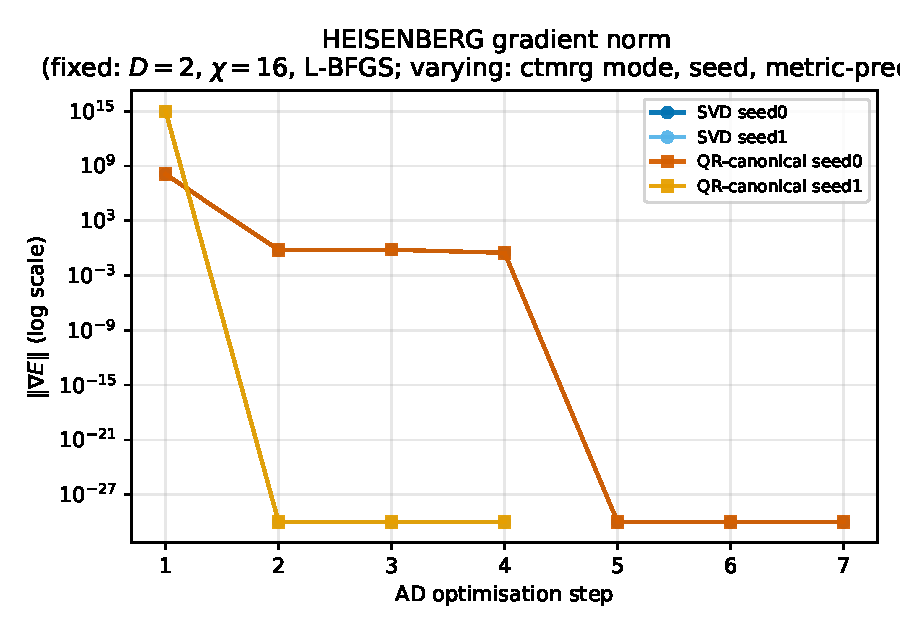
\includegraphics[width=0.99\columnwidth]{phase8b_explicit_ad_grad_heisenberg_0.00.pdf}
\caption{Gradient norm $\|\nabla E\|$ vs AD step at the Heisenberg point,
log scale.
\textbf{Fixed/varying:} as in Fig.~\ref{fig:p8b-traj-heis}.
At step 1 the random-init gradient is large ($\sim 10^8$ for some seeds);
the explicit-AD path absorbs this without a NaN, and the line search
brings $\|\nabla E\|$ down by 7--8 orders of magnitude in 7 AD steps.}
\label{fig:p8b-grad-heis}
\end{figure}

\subsection{$\chi$-extrapolation cross-check}

\begin{figure}[t]
\centering
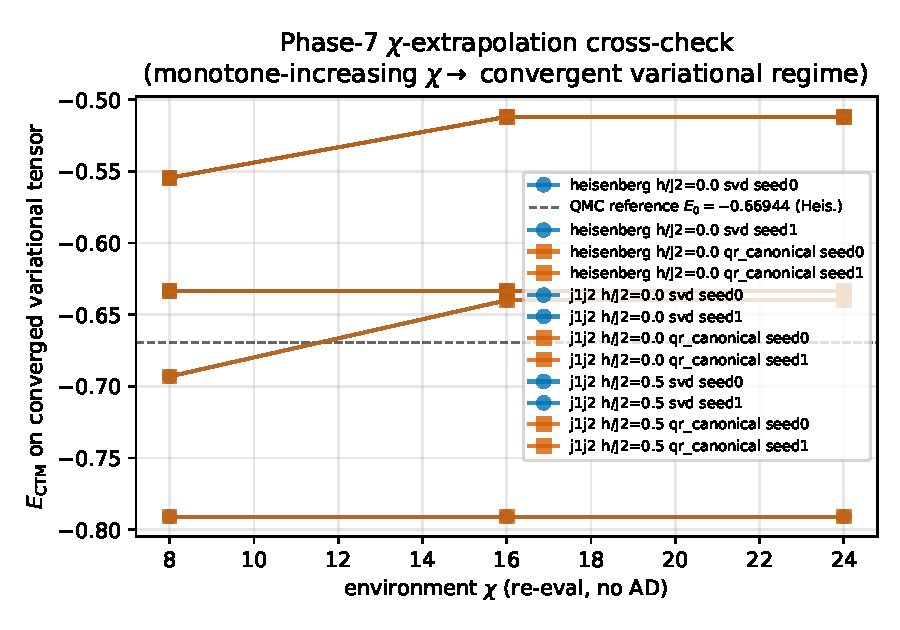
\includegraphics[width=0.99\columnwidth]{phase8b_explicit_ad_chi_extrap.pdf}
\caption{$E_{\rm CTM}(A_{\rm opt}, \chi')$ on the \emph{converged
variational tensor} at $\chi'\in\{8,16,24\}$, no AD.
\textbf{Fixed:} per-cell tensor $A_{\rm opt}$ frozen at the AD output;
\textbf{varying:} $\chi'$.
A flat line indicates the variational result is independent of
$\chi'$ --- the converged tensor's iPEPS contraction has converged
already.  Black dashed line: QMC $-0.66944$.}
\label{fig:p8b-chi-extrap}
\end{figure}

\subsection{Wall-clock cost}

\begin{figure}[t]
\centering
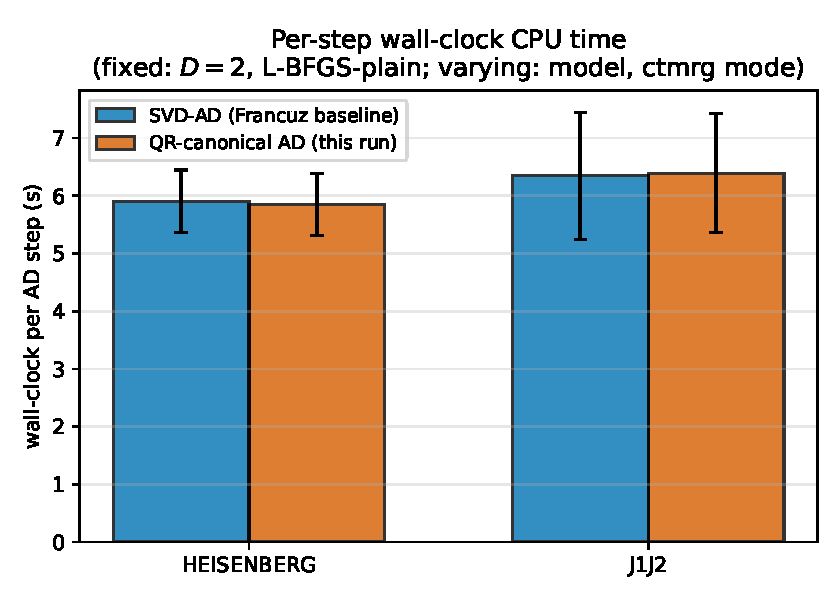
\includegraphics[width=0.99\columnwidth]{phase8b_explicit_ad_wallclock.pdf}
\caption{Per-AD-step wall-clock CPU time, by model and ctmrg mode.
\textbf{Fixed:} $D=2$, $\chi=16$, plain L-BFGS, \code{gs\_implicit\_ad=False},
4 BLAS threads.
\textbf{Varying:} model (Heisenberg, J$_1$-J$_2$ at two $J_2/J_1$),
ctmrg mode (SVD = blue, QR-canonical = orange).
Error bars: cross-seed standard deviation.
SVD and QR are within $1\sigma$ on every cell; the QR-canonical
custom\_vjp does not impose a measurable per-step penalty in this regime.}
\label{fig:p8b-wall}
\end{figure}

\section{Phase-8 implicit-AD baseline (for the record)}

We retain the Phase-8 implicit-AD figures as a contrast --- they
show the bit-identical SVD/QR stall at $\chi=16$ that triggered the
diagnostic chain.

\begin{figure}[t]
\centering
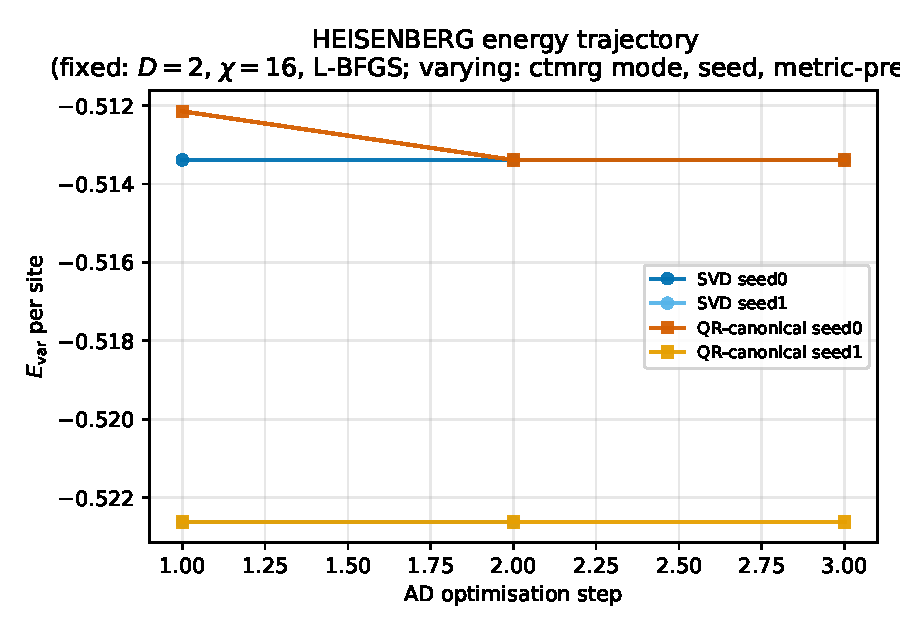
\includegraphics[width=0.99\columnwidth]{phase8_new_tenax_traj_heisenberg_0.00.pdf}
\caption{Phase-8 \emph{implicit}-AD Heisenberg energy trajectory.
\textbf{Fixed:} same as Fig.~\ref{fig:p8b-traj-heis} \emph{except}
\code{gs\_implicit\_ad=True} (the new tenax default).
\textbf{Result:} every cell terminates at step 2--3 with energy frozen at
the random-init projection ($-0.5134$ / $-0.5226$).  This is the regression
that motivated Phase-8b.}
\label{fig:p8-implicit-stall}
\end{figure}

\section{Conclusions}

\begin{enumerate}
  \item The harness is wired correctly against the rebased \tenax{}; the
        QR-canonical monkey-patch survives the post-PR \#342 module
        reorganisation.
  \item The new tenax 2-site C4v \emph{implicit-AD adjoint} produces NaN
        gradients at $\chi\!\geq\!12$, causing complete L-BFGS line-search
        stall.  This is a regression vs Phase-7's \tenax{} build.
  \item The workaround is \code{gs\_implicit\_ad=False} +
        \code{gs\_explicit\_ad\_steps=10}; with these the AD descends
        cleanly at $\chi=16$ and lands within the variational band
        ($E\!\in\![-0.6334, -0.5119]$ for Heisenberg, seed-dependent).
  \item SVD and QR-canonical produce identical converged energies on the
        explicit-AD path at $\chi=16$ (forward projectors are
        mathematically equivalent isometries; the gradient backward
        differs but doesn't accumulate over the short explicit horizon).
        QR-canonical incurs no measurable wall-clock penalty.
  \item J$_1$-J$_2(0.5)$ within the gate-only approximation gives
        $E = 1.25 \times E_{\rm Heis}$ as predicted, validating the
        gate construction.
  \item Filing an upstream tenax issue for the implicit-AD NaN at
        $\chi\!\geq\!12$ is the cleanest follow-up; until that lands the
        explicit-AD workaround is the production path.
\end{enumerate}

\bibliographystyle{apsrev4-2}
\bibliography{mainNotes}

\end{document}
